\documentclass[conference]{IEEEtran}
\IEEEoverridecommandlockouts

\usepackage{cite}
\usepackage{amsmath,amssymb,amsfonts}
\usepackage{graphicx}
\usepackage{textcomp}
\usepackage{xcolor}
\usepackage{float}
\usepackage{multirow}
\usepackage{booktabs}
\usepackage{hyperref}

\begin{document}

\title{Automated Vision-Based Bolt Handling for Industrial Applications Using a Manipulator\\
\thanks{* Authors contributed equally to this work.}
\thanks{SMME: School of Mechanical and Materials Engineering.}
\thanks{CAIR: Center for Artificial Intelligence and Robotics.}}

\author{\IEEEauthorblockN{Surya Prakash S.K\textsuperscript{*}}
\IEEEauthorblockA{\textit{SMME, Research Scholar} \\
\textit{IIT Mandi}\\
Mandi, India \\
s.surya1754@gmail.com}
\and
\IEEEauthorblockN{Amit Shukla}
\IEEEauthorblockA{\textit{Chairperson CAIR} \\
\textit{IIT Mandi}\\
Mandi, India \\
amitshukla@iitmandi.ac.in}
\and
\IEEEauthorblockN{Smrithi S\textsuperscript{*}}
\IEEEauthorblockA{\textit{CAIR, Research Intern} \\
\textit{IIT Mandi}\\
Mandi, India \\
smrithisiddagangaiah@gmail.com}
}

\maketitle

\begin{abstract}
Fasteners are critical components in industrial assembly processes. Accurate identification and size estimation of fasteners are essential for enhancing the efficiency and precision of these processes. However, the detection and segmentation of fasteners in factory environments are challenging due to their limited visual features and frequent overlap. This paper presents a novel approach for automated bolt handling using 3D point cloud data acquired from an RGB-D camera. Our method employs k-means clustering for segmentation and Oriented Chamfer matching for precise pose estimation, enabling a 6-DOF robotic arm to accurately pick and place bolts. Color-based segmentation and contour analysis facilitate size estimation for subsequent sorting. Experiments conducted in a simulated shop floor environment using Gazebo (ROS1) with a Kinova Gen3 Lite arm demonstrated the system's ability to handle overlapping bolts and achieved bolt sorting without any miss-classifications. This research contributes to enhanced automation and productivity in industrial automation, with potential applications in various industries requiring precise component handling, such as automotive, aerospace, and electronics.
\end{abstract}
\begin{IEEEkeywords}
Industrial Automation, Vision-Based Automation, Factory Automation, Automation Assembly, Warehouse Management, Object Detection and Segmentation, Size Estimation, Template Matching.
\end{IEEEkeywords}

\section{Introduction}
Efficient object manipulation with robots is a crucial component of modern industrial automation. Precise object detection, size estimation, and sorting are essential for various processes, including component assembly, packaging, and quality control. In particular, sorting small, low-textured objects in densely packed environments, common in warehouses, assembly lines, and logistics operations, remains a significant challenge. Manual sorting is labor-intensive, error-prone, and can lead to production bottlenecks. Inaccurate sorting can result in delayed production, increased costs, and reduced overall efficiency. Existing research on object sorting often faces limitations in handling densely packed objects with limited visual features. This paper addresses these challenges by presenting a novel vision-based approach for automated bolt handling. 

% Efficient object manipulation is a cornerstone of modern industrial automation. Accurate object detection and size estimation are critical for optimizing processes such as sorting, assembly, and packaging. 
 
Existing methods for object sorting often suffer from limitations in terms of accuracy, speed, and adaptability to complex environments. Many approaches require multiple sensor equipment, increasing system complexity and cost. To address these challenges, this paper presents a novel approach for localizing bolts in overlapping configurations using RGB-D data and template matching. Our method leverages the rich information provided by RGB-D cameras to improve object detection accuracy and reduce reliance on multiple sensors. By addressing the limitations of current methods, our proposed technique aims to enable more robust and efficient automation systems.

Present paper is structured as following, the introduction in Section I, Section II provides a comprehensive review of related work in the field of template matching, especially for low-textured objects, and size estimation using RGB-D information. Section III details the proposed methodology for localization of the bolts with respect to the base frame of the robotic arm, size estimation and sorting. Section IV discusses the results, and Section V draws conclusions based on the results obtained.

\section{Related Work}
Recent advancements in computer vision techniques have garnered significant attention from researchers, leading to substantial contributions in the fields of object detection and object pose estimation. In \cite{MITPAPER}, K. Ikeuchi et al. pioneered the use of photometric stereo and the Extended Gaussian Image for robust hand-eye coordination in bin-picking. Their system effectively segmented the scene using the needle map and determined object orientation, enabling successful object picking. While this work laid a foundation for bin-picking, its practical applicability is limited by its reliance on specific lighting conditions and the computational complexity of the approach. Further, Krisnawan Rahardja and Akio Kosaka in \cite{2NDPAPER}, addressed the challenges of bin-picking for complex industrial objects by employing a vision-based approach that utilized stereo vision and simple object features to reduce computational complexity.
 Their algorithm achieved high success rates in object detection and pose estimation. However, the system's autonomy was limited by the lack of grasping experiments and the reliance on human intervention for robot manipulation. While this work demonstrated the potential of using simple features for efficient bin-picking, it did not fully address the end-to-end process of object grasping and placement. In \cite{3D_object_recognition_in_cluttered_environment_using_stereo_vision}, Sumi et al.  used stereo vision to determine the 6 DOF pose of an object placed in cluttered scene, even when undergoing occlusion. They demonstrated good accuracy in estimating the pose and improving recognition rates. However, their work faces challenges related to computational complexity and limited to certain lighting conditions. In
\cite{Segmentation_driven_6D_pose} Yinlin Hu et al.
 introduced a novel segmentation-driven approach for 6D pose estimation. By predicting 2D keypoint locations for visible object parts and combining them using confidence scores, the method achieved robust pose estimation. This approach demonstrated state-of-the-art performance on challenging datasets like Occluded-LINEMOD and YCB-Video. However, its reliance on accurate segmentation and potential sensitivity to occlusions and initial conditions remain limitations.

Surface texture is a crucial feature for object recognition, but many industrial components lack distinctive textural patterns. Paul Wohlhart et al. in their work\cite{Learning_descriptors}, proposed learning descriptors using CNN to address this challenge. Their approach demonstrated potential for pose information but had high computational complexity and a strong reliance on the dataset. Moreover, the method's robustness was compromised by lighting variation, occlusions, and background clutter, affecting descriptor accuracy. In \cite{Segmenting_Unseen_Industrial_Components} Seunghyeok Back et al proposed a synthetic data generation pipeline and an RGB-D Fusion Mask R-CNN to address the segmentation of texture-less industrial components. By randomizing textures in synthetic data, the focus shifted to shape-based features. A confidence map estimator enhanced the model's ability to exploit depth information for improved segmentation. While this approach demonstrated promising results, the reliance on synthetic data for training raised concerns about domain adaptation to real-world scenarios. Various self-supervised for segmentation and data extraction as presented in \cite{shapematcher} are also being developed for various downstream task like robotic grasping. However, developing deep learning models will be extensive and time-consuming. 

Shape-based object segmentation can be advantageous in scenarios with poor figure-ground contrast or illumination, as shown in \cite{Shape_guided_object_segmentation}. While the framework performs well on the shapes it has been trained on, its ability to generalize to completely unseen shapes might be limited. Walter Wohlkinger et al. viewed the classification task as a matching problem. Their work \cite{Shape_based_depth_image_to_3D} introduced a method that identifies similar 3D models from comparable viewpoints by analyzing specific surface features. Although the method incorporates inter-view similarity, it may still struggle with extreme variations in viewpoints. Objects viewed from angles significantly different from those in the training set might not be matched accurately. The approach might also have limitations in handling severe occlusions where significant parts of the object are not visible in the depth image. This can affect the accuracy of matching and classification. Most bin-picking applications have utilized the concept of matching a template of the expected object in the scene to estimate its 3D pose, as it is simpler and does not require any previously trained models. This methodology can be preferable in industries because the CAD models used as templates are expected to be present within the setup \cite{Fast_Object_Pose}. Although the method shows promising results in terms of speed, integrating it into real-time applications might require further optimization, especially for handling a wide variety of objects in diverse conditions. Further \cite{Mobile_bin_picking_with_an_anthropomorphic_service_robot} is one other example where such method is employed. \\

Depth-image-based segmentation can be much simpler, as indicated in \cite{A_study_on_picking_objects_in_cluttered}. The depth edge represents the contours of depth images, but normally depth images tend to have low resolution. The accuracy of the depth features and the picking performance depends on the quality and resolution of the depth sensor used. To improve the resolution and obtain better results, Xinyu Wang et al. propose in their paper \cite{LBP_based_edge_detection} a novel edge detection method with high accuracy and computational speed that even outperforms renowned edge detection methods. In highly complex scenes with multiple overlapping objects, the method might struggle to accurately detect edges, especially if the objects have similar depth values. 

Recently, point cloud-based segmentation has become more preferred. \cite{fast_and_robust_bin_picking} Used point clouds and improved density-based spatial clustering of applications with noise (DBSCAN). By combining it with the region-growing algorithm and using Octree, they have attempted to speed up the calculation but the accuracy of object detection and pose estimation depends on the quality and resolution of the sensors used. Although RGB images can be used for pose estimation, as shown in \cite{templates_for_3D}, a deep learning architecture might be required to get better results. 
\\Production environments and assembly line applications often encounter unsorted components of varying sizes, such as metric bolts, where size can be a criterion for differentiation \cite{Development_of_machine_vision}. Size estimation in real time can also be achieved using classical vision and RGB-D data without the need for extensive model development, as demonstrated by \cite{On_tree_mango_fruits} and \cite{Real_time_object_measurement}. Standard benchmarking protocols, especially those targeted at bin-picking tasks, are developed to test such systems. \cite{MorganPaper} and \cite{Evaluating_robot_bin_picking_performance} have presented some of these methods. In \cite{Fast_object_localization}, Liu et al. presented a practical vision-based robotic bin-picking system that performs object detection and localization in heavy clutter using Fast Direction Chamfer Matching (FDCM). This system showed remarkable performance compared to existing shape-matching algorithms by using specialized hardware Multi-flash camera (MFC) and Multi camera System which produced robust depth images. The FDCM improves the accuracy of traditional chamfer matching by including orientation of the edges and increasing the matching speed by approximating the edges.

In our paper, we use pose error and sorting success rate to evaluate our methodology. Without requiring specialized equipment, the robotic arm can perform detection, pick-up operations, and sorting of bolts based on their sizes under varying lighting conditions. Additionally, we can sort bolts of varying sizes using a single median template, eliminating the need for a large database. Moreover, the methodology can be easily adapted to other components by simply modifying the CAD model, making it a versatile solution for various industrial automation tasks.

\section{Methodology}
To demonstrate the algorithm's effectiveness for automated bolt sorting from overlapping configurations,
 an industrial shop-floor environment was created in the Gazebo ROS1 simulation platform, as shown in Fig. \ref{setup}. The setup included bolts of varying sizes in random overlapping configurations placed in a bin, simulating a cluttered environment where the algorithm must be capable of distinguishing individual bolts. Manipulation operations were carried out using the GAZEBO model of the Kinova Gen3 Lite, a 6-DOF serial manipulator. A globally positioned Open-Kinect camera was used to obtain RGB-D images of the scene. Conventional techniques using template matching for object detection search the entire sample space to find a suitable pattern.
 In our algorithm, we utilize the RGB image a priori to determine search volumes occupied by bolts. This is achieved by segmenting the image using k-means clustering and then applying a binary threshold.
 Point cloud data corresponding to these search volumes are extracted and downsampled according to the requirements. This smaller sample space is then used for template matching with the reference template.

 Once the bolt's pose is obtained through template matching using chamfer distance calculation, the robotic arm picks it up from the bin and places it under the globally positioned camera for size estimation. Based on the estimated size, the bolt is sorted into its respective bin. This process is repeated until all bolts are transferred to their respective bins.

The overall process of automated bolt sorting from a heap is divided into six distinct phases:

\begin{itemize}
\item Phase 1: RGB-D data acquisition
\item Phase 2: Segmentation of RGB Image Using k-means Clustering
\item Phase 3: Data Conditioning
\item Phase 4: Template Matching Using Chamfer-Distance Calculation
\item Phase 5: Robotic Manipulation
\item Phase 6: Size Estimation and Sorting
\end{itemize}
\begin{figure}
    \centering
    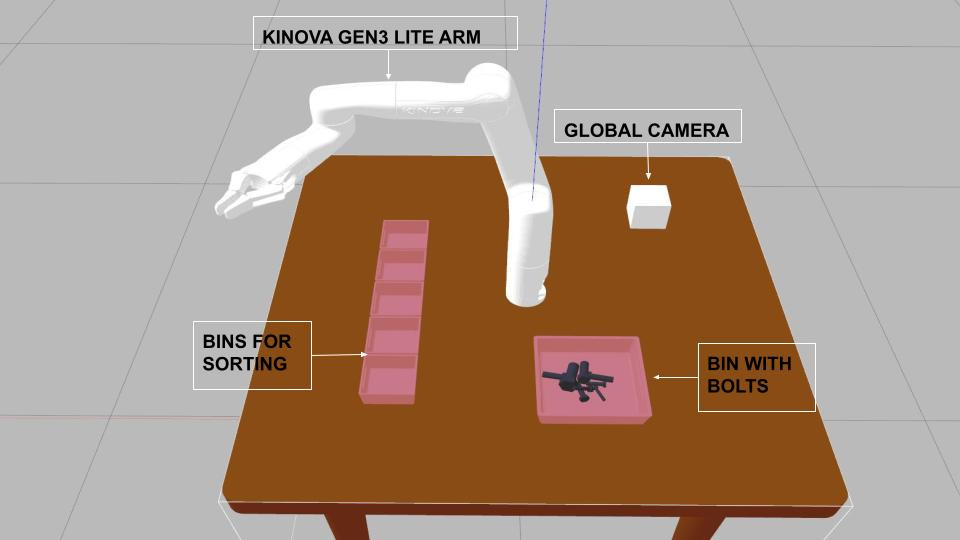
\includegraphics[width=0.8\linewidth]{Robotic_arm_setup.jpg}
    \caption{Experimental Setup in Gazebo Environment}
    \label{setup}
\end{figure}

The detailed explanation of the methodology is presented in the following subsections.
\subsection{\textnormal{\textbf{Segmentation of RGB Image Using k-means Clustering}}}

The global camera captures RGB-D data of the scene, from which point cloud data is extracted. For segmentation, k-means clustering is applied to the RGB image assuming three clusters: table, bin, and bolts. k-means clustering groups the pixels, based on their intensities into the number of clusters specified. On application of k-means a segmented image distinguishing bolts from the rest of the scene is obtained. The segmented image is then converted to a binary image to obtain the contours of the bolts. This step provides individual contours and identifies the corresponding bolts in the image. A flowchart indicating various steps in the phase is shown in Fig. \ref{segmentation}.
\begin{figure}
\centering
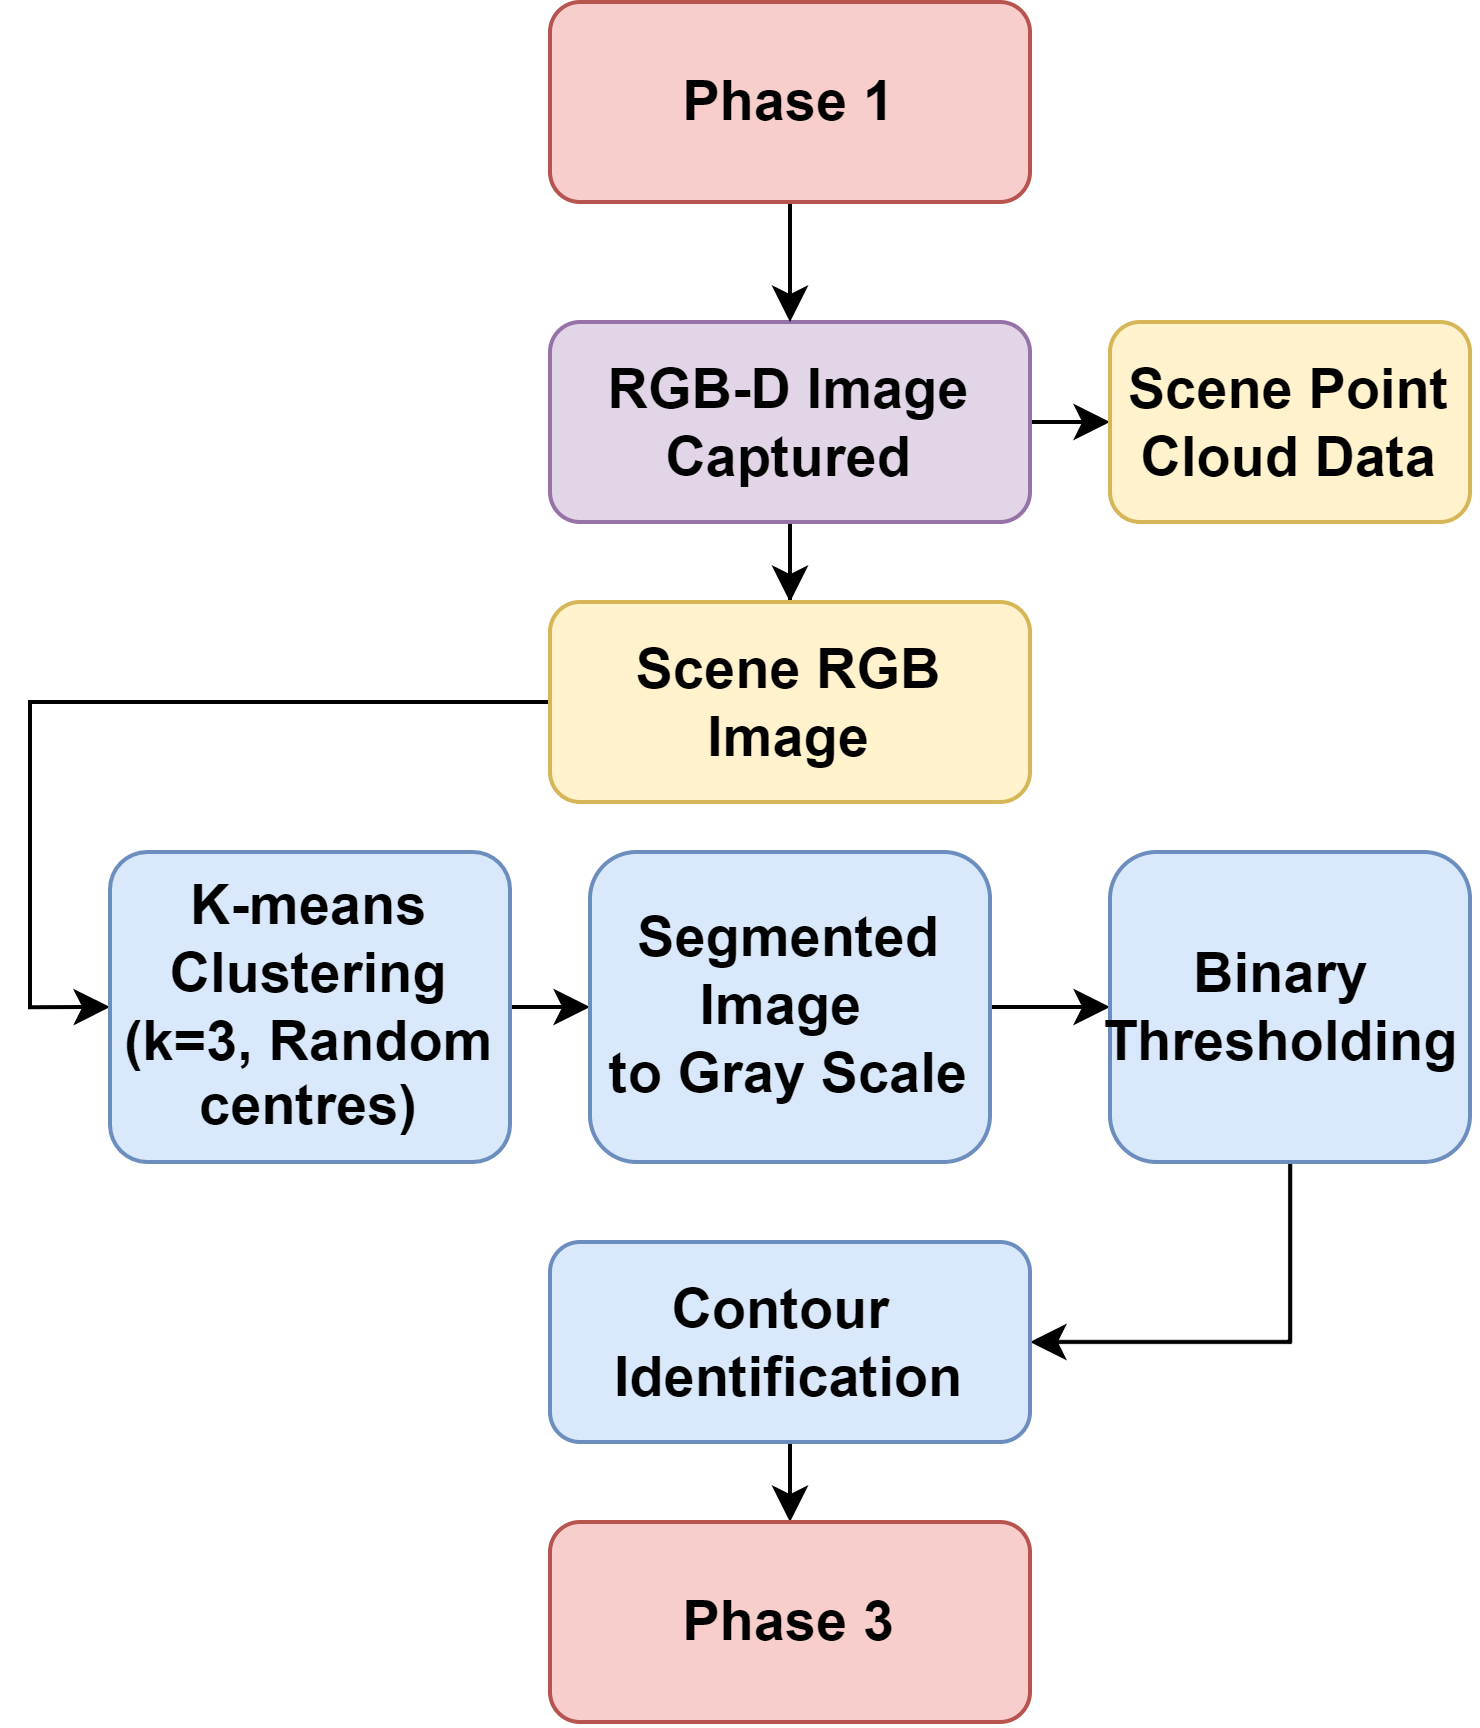
\includegraphics[width=0.6\linewidth]{Phase2.png}
\caption{Segmentation of the Captured RGB Image}
\label{segmentation}
\end{figure}

\subsection{\textnormal{\textbf{Template Matching Using Chamfer Distance Calculation}}}
Template matching follows a nested brute-force approach. The steps involved are outlined as follows and are illustrated in Fig. \ref{search_vol}.
\begin{itemize}
    \item \textbf{Extracting Search Volume }
    \newline From the detected contours, the first contour is selected for template matching. A minimum area rectangle is used to draw the bounding box around the contour, defining the area of interest in the point cloud data (PCD). The PCD is then downsampled using the Voxel Grid filter to reduce computational complexity and is stored for further processing.
    \item \textbf{Translating the Template Onto Bolt Point Cloud Data}
    \newline The center of the template is translated to position 'j' in the object PCD. The corresponding position vector is denoted as $\textnormal{P}_{j,s}$.
    \item \textbf{Rotating the Template in the Scene}
    \newline Once the center of the template is translated to the position of the $\textnormal{j}^{\text{th}}$ point in the scene, it is incrementally rotated from 0 to 360 degrees for both yaw and pitch angles. For every combination of yaw angle $\theta$ and pitch angle $\delta$, the Chamfer distance is calculated. If the number of points in the template PCD is N, the Chamfer distance $\textnormal{D}(p_{j,s},\theta,\delta)$ is the sum of the distances from each point in the template to its nearest neighbor in the scene. Here, $\textnormal{p}_{i,t}$ is the position of the $\textnormal{i}^{\text{th}}$ point in the template, and $\textnormal{c}$ corresponds to the position of its nearest neighbor in the scene PCD. For each angle combination, the sum of the minimum distances is calculated as shown in Eq. \ref{chamfer_eq} and stored. This process is repeated for every position $\textnormal{j}$ in the template PCD. The minimum of $\textnormal{D}(p_{j,s},\theta,\delta)$ from these stored values is extracted (as shown in Eq. \ref{minD}), and the corresponding feature vector in Eq. \ref{featv} obtained from Fig. \ref{Template_matching},  further subjected to projective transformations to localize bolt from image coordinates to Cartesian coordinates in camera frame.
\end{itemize}
\begin{figure}
    \centering
    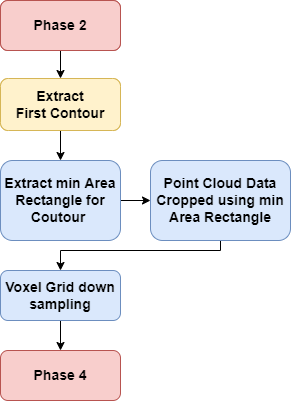
\includegraphics[width=0.5\linewidth]{Phase3.png}
    \caption{Obtaining Search Volume from the Captured Scene}
    \label{search_vol}
\end{figure}
\begin{equation}
\textnormal{D}(p_{j,s},\theta,\delta) = \sum_{i=0}^{N} |(\textnormal{p}_{i,t} - \textnormal{c})^2|  \label{chamfer_eq}
\end{equation}
\begin{equation}
{\textnormal{D}(P_{j,s},\theta,\delta)} = \textnormal{min}(\textnormal{D}(p_{j,s}, \theta, \delta))  \label{minD}
\end{equation}
\begin{equation}
\textnormal{V} = (\textnormal{P, } \theta, \delta) \label{featv}
\end{equation}
Fig. \ref{Object_pose_fc} and Fig. \ref{Robotic_manipulation_fc} indicate the algorithm used for template matching. 

\begin{figure} 
    \centering
    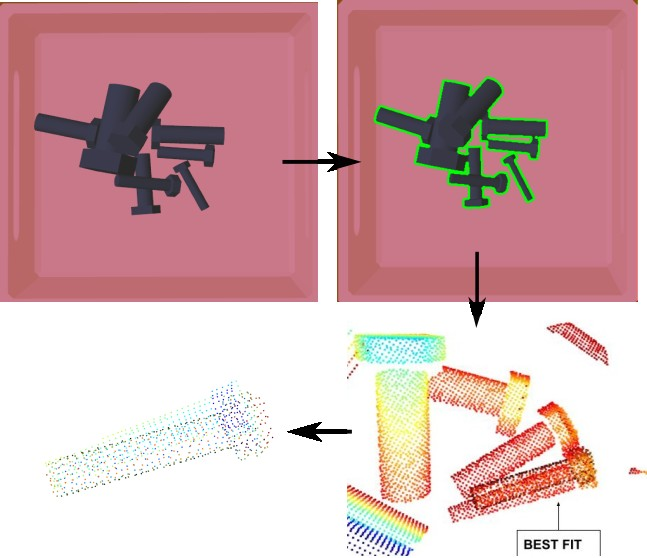
\includegraphics[width=0.7\linewidth]{Template_matching.jpeg}
    \caption{Match Found in Overlapping Configured Bolts in bin}
    \label{Template_matching}
\end{figure}
\begin{figure} 
    \centering
    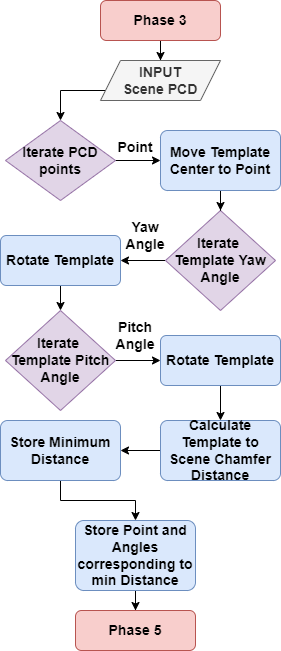
\includegraphics[width=0.5\linewidth]{Phase4.png}
    \caption{Rotational Pose($\theta$, $\delta$) Estimation of the Bolt in the Bin}
    \label{Object_pose_fc}
\end{figure}
\begin{figure}
    \centering
    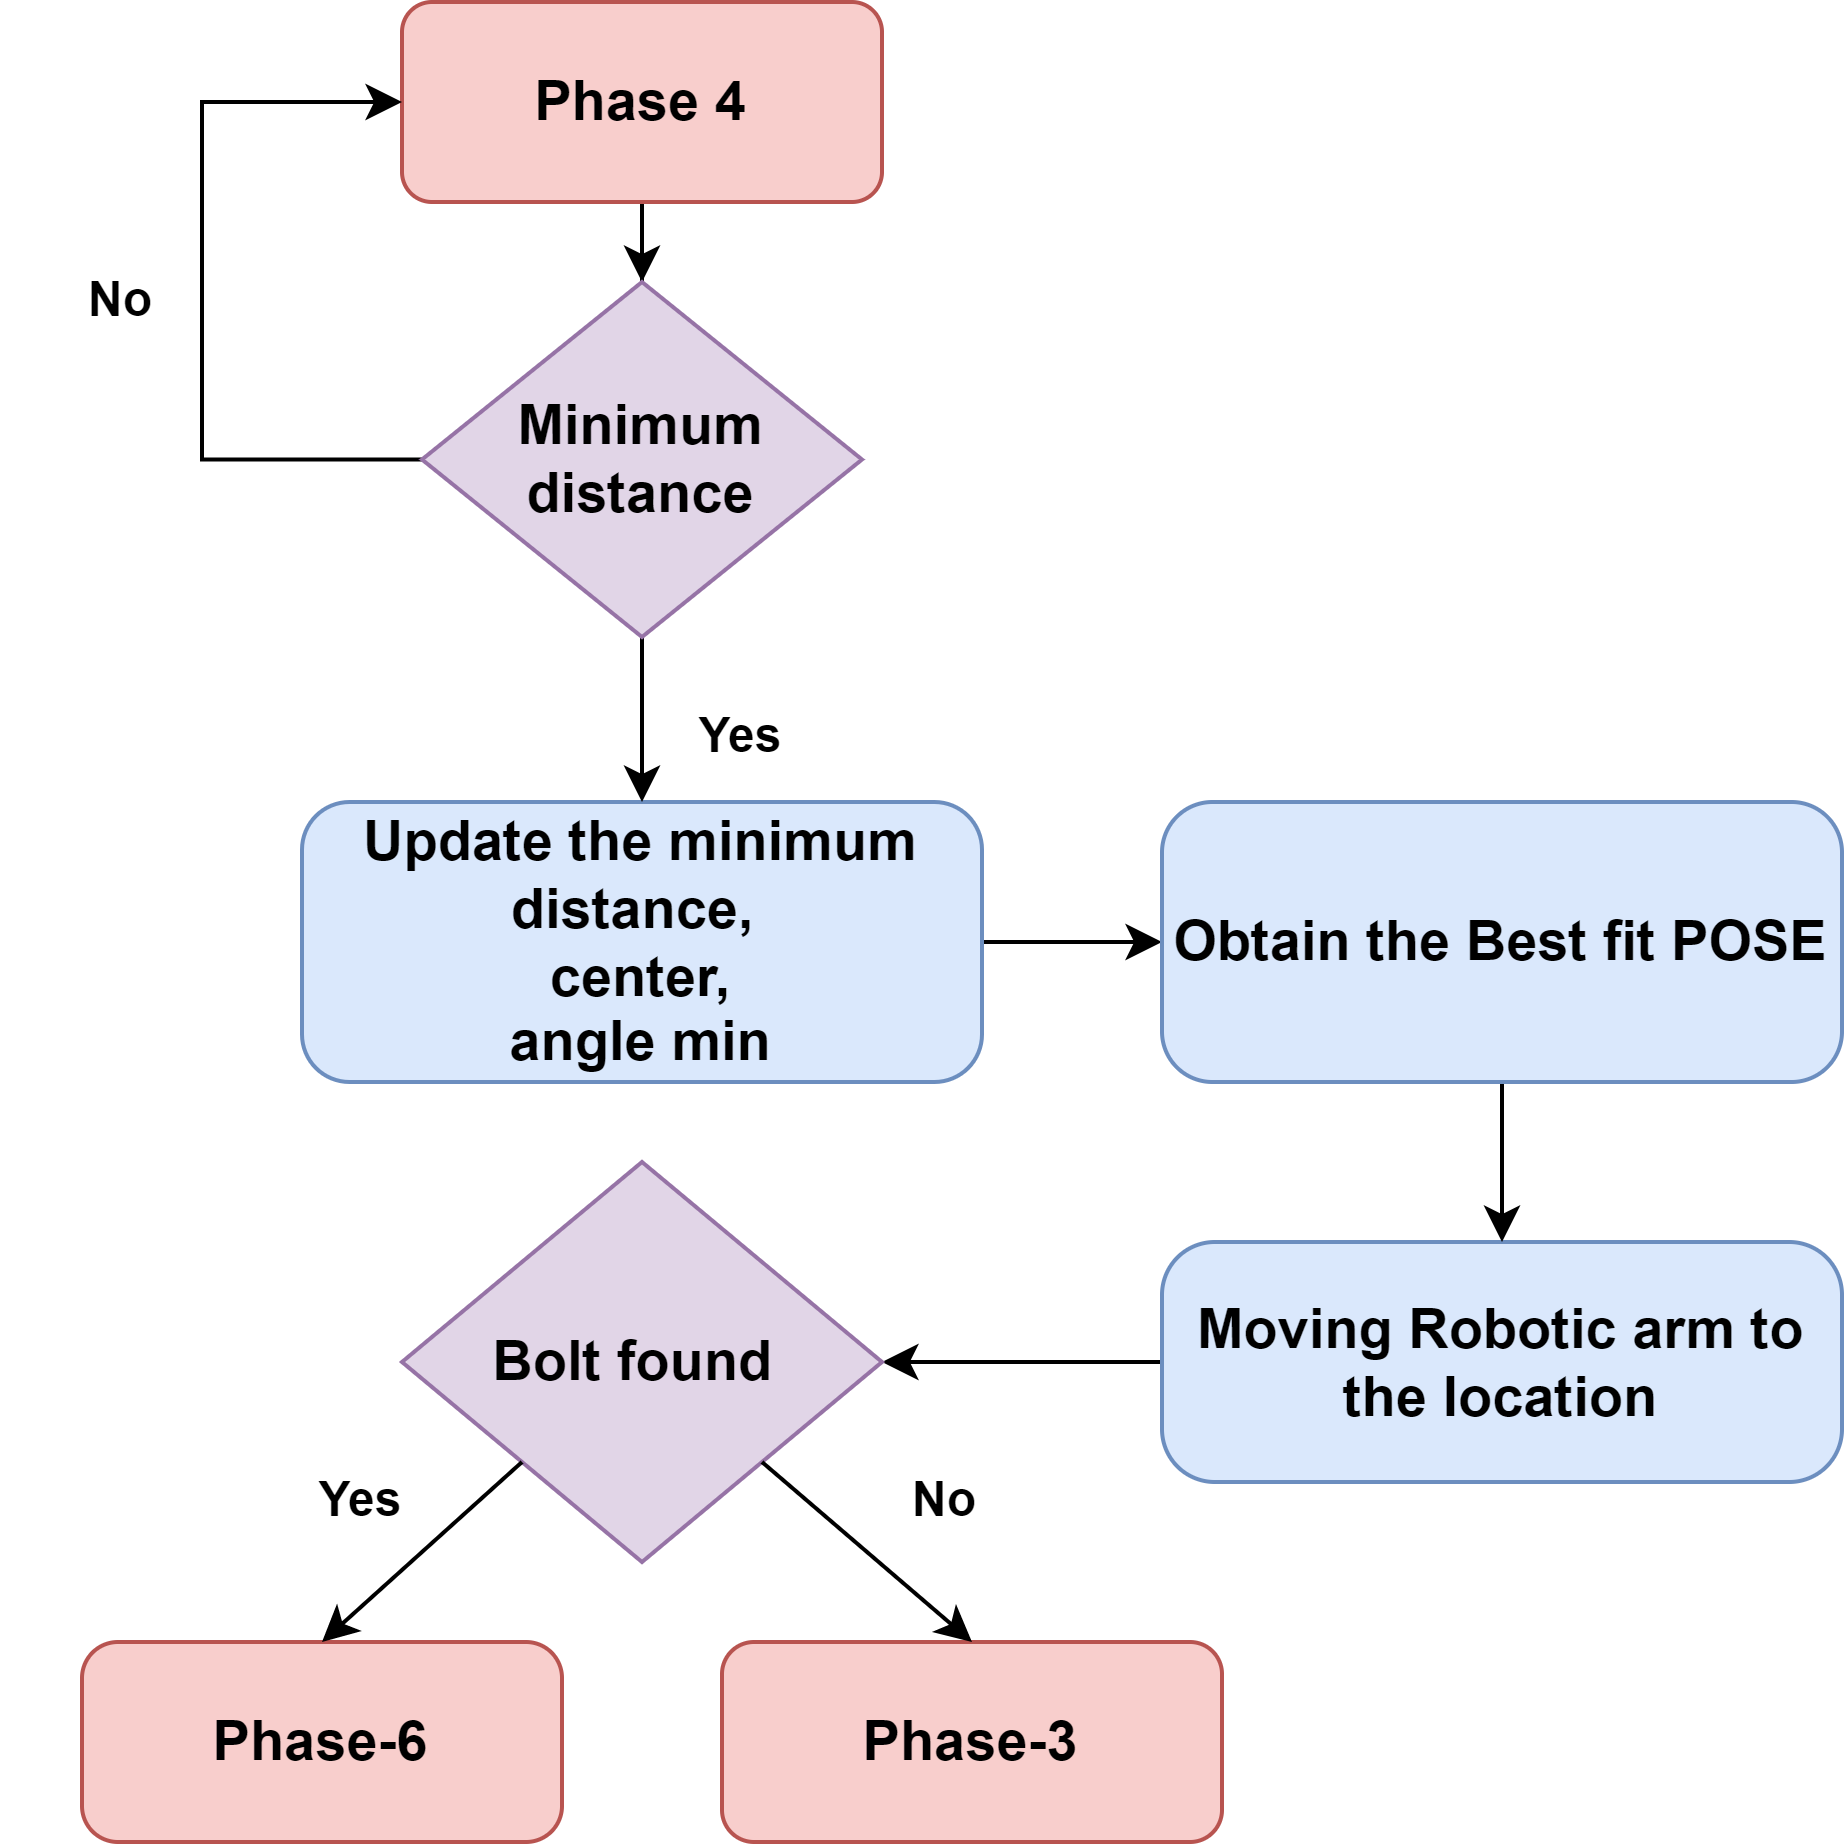
\includegraphics[width=0.7\linewidth]{Phase5.png}
    \caption{Robotic Arm Movement to bin for picking up the detected bolt}
    \label{Robotic_manipulation_fc}
\end{figure}
\subsection{\textnormal{\textbf{Localization of the Bolt with respect to the Robot Base Frame}}}  
The feature vector $\textnormal{V}$ consists of the position vector of the bolt and the angles related to its orientation in the camera frame. To transform it to the base frame of the robotic arm, Eq. \ref{transformation} is used, where the rotation matrix of the bolt with respect to the camera, $R^C_b$, is a function of ${\theta}$ and ${\delta}$. The goal orientation of the bolt with respect to the base is determined by $R^B_b$, which is a function of $R^B_C$, the orientation of the camera with respect to the base, and $R^C_b$. The position of the bolt with respect to the base, $P^B_b$, is a function of $R^B_C$, the position of the bolt in the camera frame, $P^C_b$, and the position of the camera with respect to the base. The target pose is then provided to the MoveIt interface for the picking process. Pick-and-place operations with a Kinova Gen3 Lite have been performed under various lighting conditions as shown in Fig. \ref{Diff_lighting.png}.
\begin{figure}
    \centering
    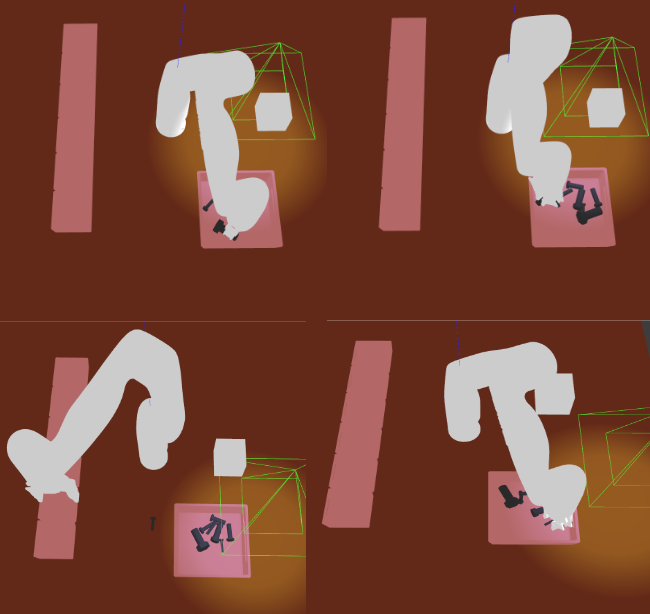
\includegraphics[width=0.7\linewidth]{Diff_lighting.png}
    \caption{Robotic Arm Performing pick-place of Bolt Under Varying Lighting Conditions}
    \label{Diff_lighting.png}
\end{figure}

\begin{equation}
\begin{bmatrix}  R^B_b & P^B_b \\ 0 & 1\\ \end{bmatrix} = \begin{bmatrix}  R^B_C \cdot R^C_b  & R^B_C.P^C_b + P^B_C \\ 0 & 1\\ \end{bmatrix} \label{transformation}
\end{equation}
\subsection{\textnormal{\textbf{Size Estimation and Sorting}}}
The bolt is placed under the global camera for size estimation, which is essential for sorting. The size estimation algorithm operates as shown in the flowchart in Fig. \ref{size_es_al}. The radius of the bolt in pixels is R calculated using the Euclidean distance from the centroid of the bolt $(c_x,c_y)$ to its nearest point on the contour $(NP_x,NP_y)$, as given in eq. \ref{size eq}. This assumes that the nearest point lies on the perpendicular from it's origin to the edge. Since the estimated diameter is in pixels$(Size_{P})$, projective transformations are used to convert it to the actual size in Cartesian coordinates$(Size_{R})$ as shown in Eqs. \ref{pinhole camera eqn} and \ref{real size}. Here, $\textnormal{res}$ refers to the resolution$, \textnormal{fov}$ refers to the field of view of the camera and F is the focal length of the camera. Conceptual review of the logic is given in Fig. \ref{sz_es}. 
\begin{equation}
\textnormal{R} = \sqrt{((\textnormal{N}P_x - \textnormal{c}_x)^2 + (\textnormal{N}P_y - \textnormal{c}_y)^2)}\label{size eq}
\end{equation}
\begin{equation}
\textnormal{Size}_P= 2 \cdot \textnormal{R}\label{dia eq}
\end{equation}\begin{equation}
\textnormal{F} = \frac{(\textnormal{res}\cdot \textnormal{depth})}{2 \cdot \textnormal{tan}(\textnormal{fov}/2))} \label{pinhole camera eqn}
\end{equation}
\begin{equation}
\textnormal{Size}_R = (\textnormal{Size}_P \cdot \textnormal{F}) \label{real size}
\end{equation}

\begin{figure}
    \centering
    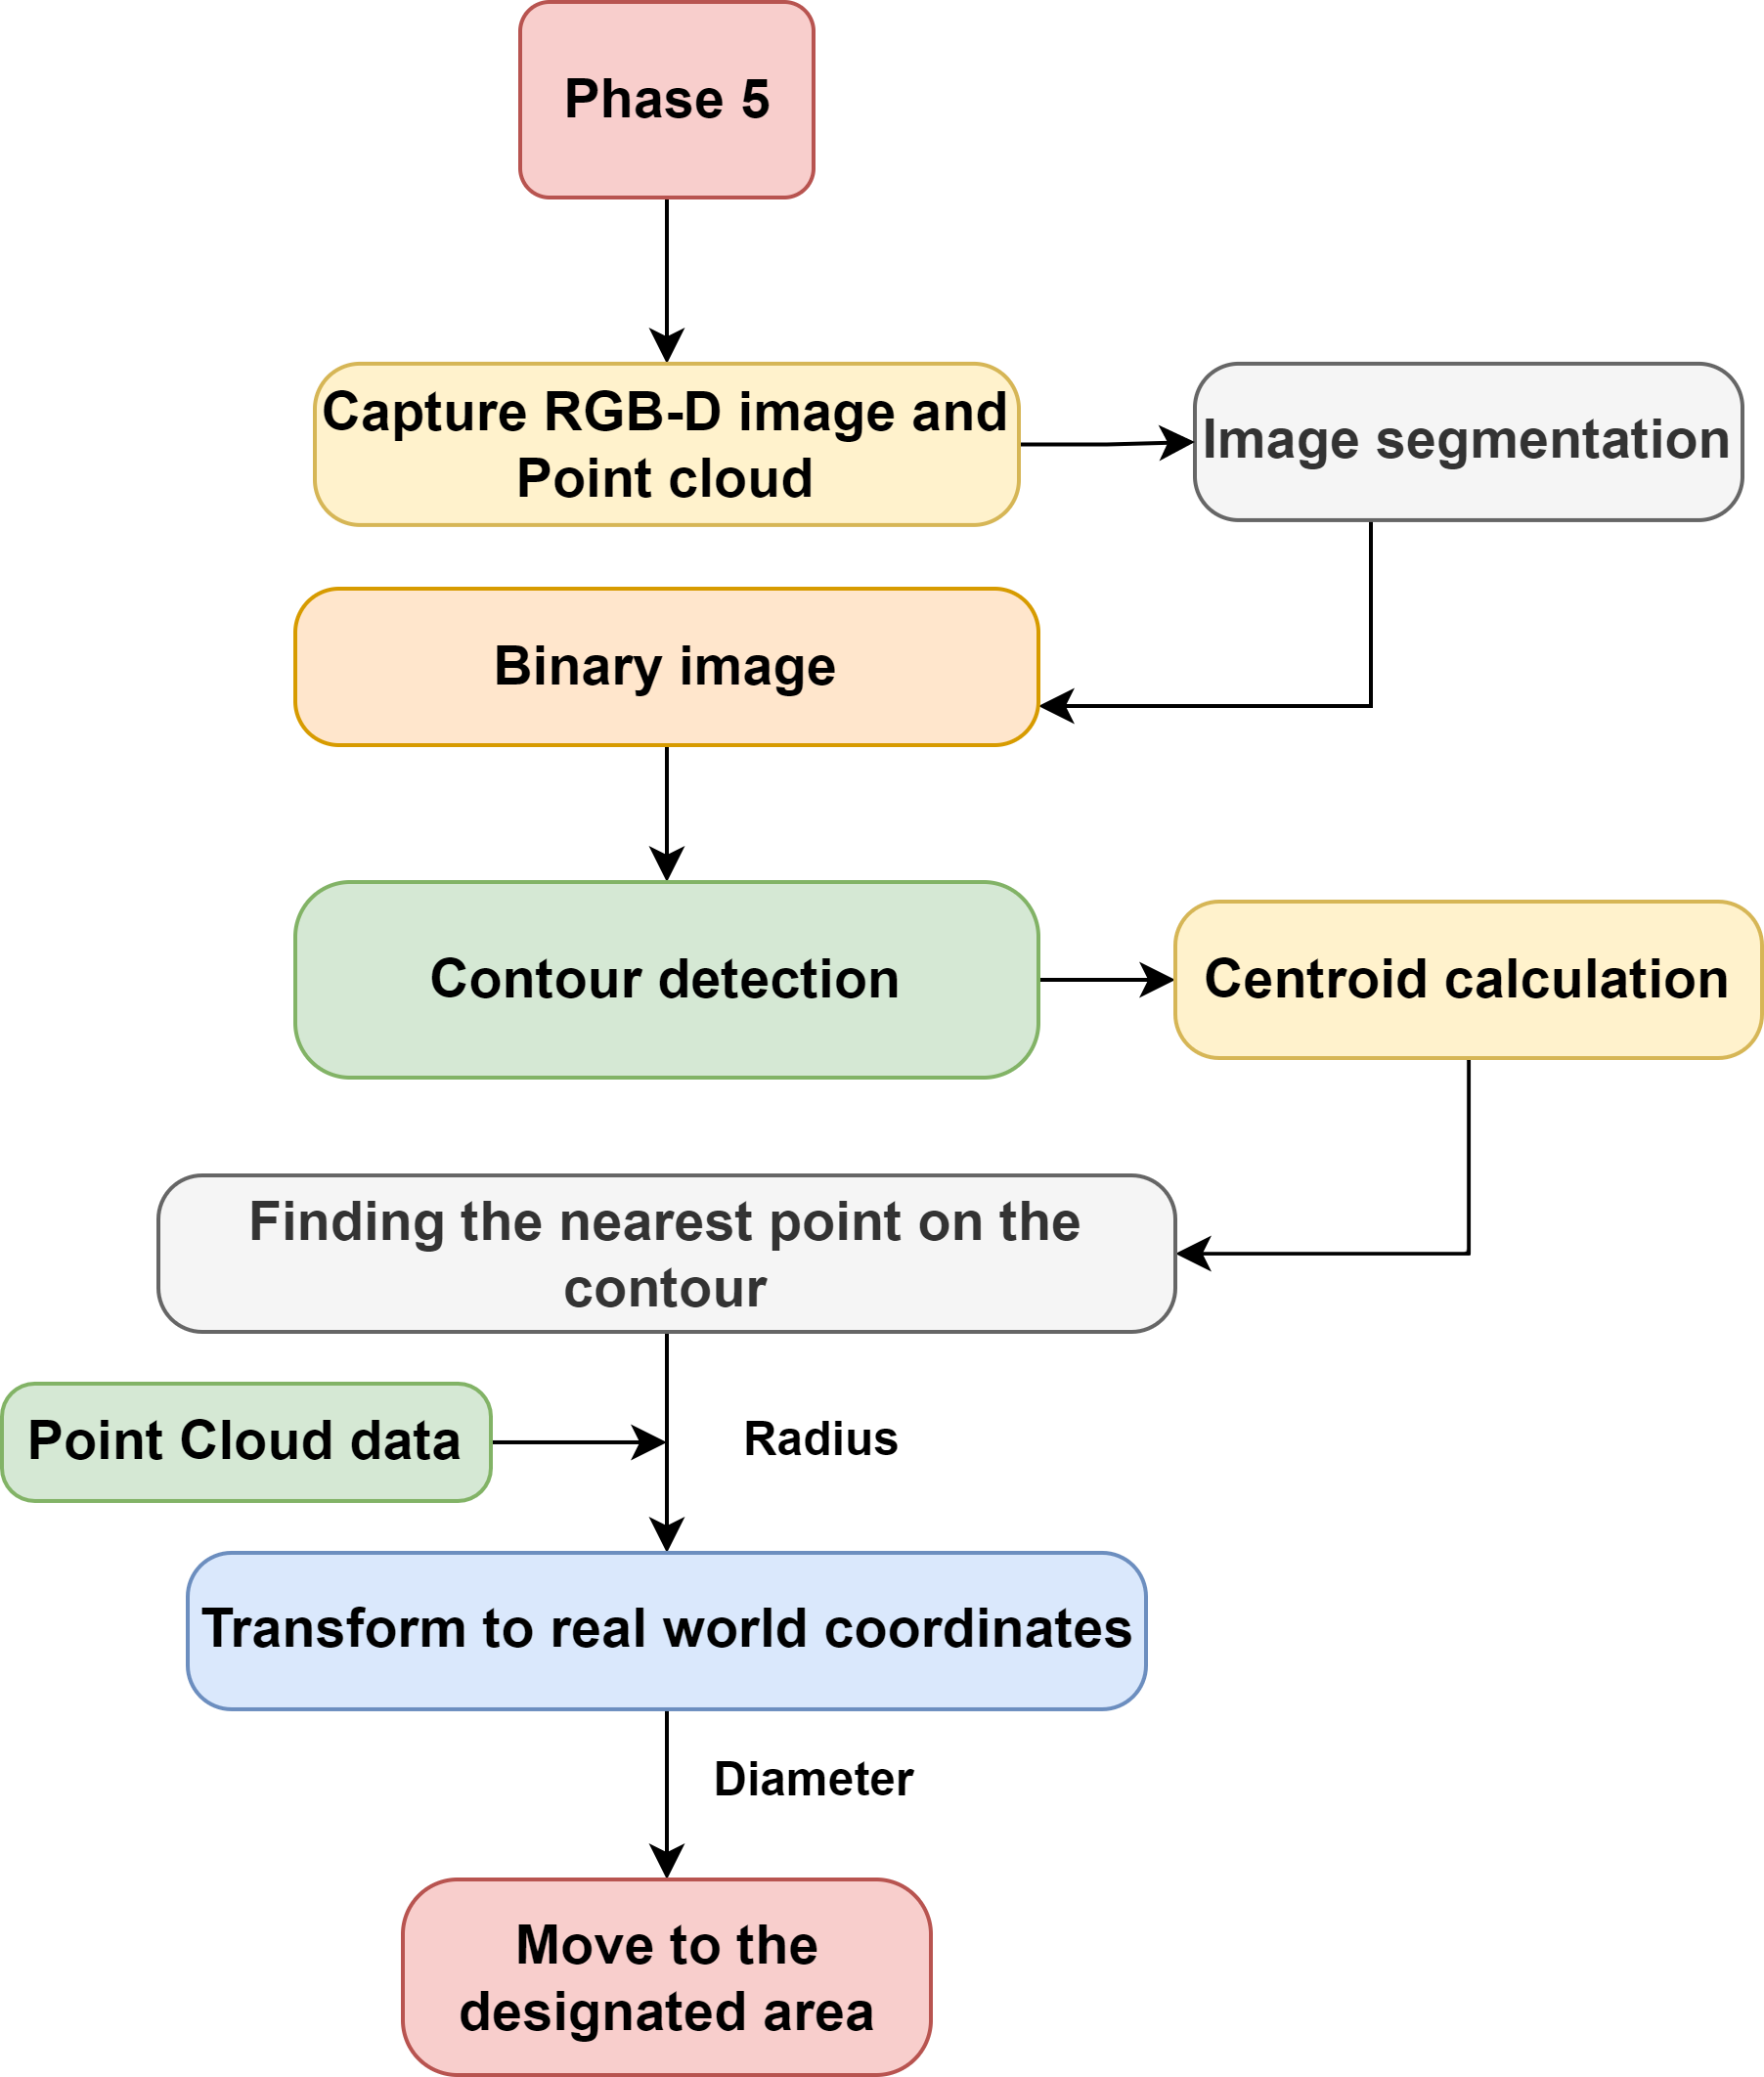
\includegraphics[width=0.8\linewidth]{Phase6.png}
    \caption{Bolt Size Estimation Algorithm}
    \label{size_es_al}
\end{figure}
\begin{figure}
    \centering
    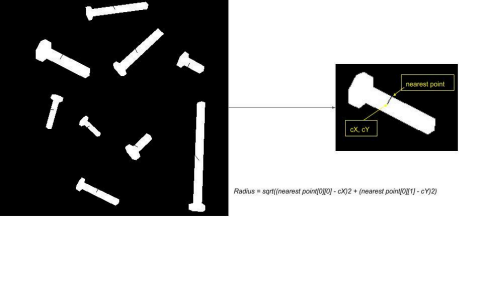
\includegraphics[width=1.0\linewidth]{Binary image.png}
    \caption{Size Estimation of Bolts Detected from Bin}
    \label{sz_es}
\end{figure}
\section{Results and discussion}

\begin{table}[ht]
\caption{Table representing position error}
\centering
\resizebox{\columnwidth}{!}{%
\begin{tabular}{|l|c|c|c|}
\hline
\begin{tabular}[c]{@{}l@{}}Metric\\ Bolt\end{tabular} & \begin{tabular}[c]{@{}c@{}}Actual position \\ (in m)\end{tabular} & \begin{tabular}[c]{@{}c@{}}Estimated Position\\ (in m)\end{tabular} & \begin{tabular}[c]{@{}c@{}}Error in distance\\ (in m)\end{tabular} \\ \hline
M6  & {[}-0.110 0.250 0.553{]}  & {[}-0.109 0.249 0.557{]}  & 0.004  \\
M8  & {[}-0.122 0.246 0.556{]}  & {[}-0.121 0.249 0.558{]}  & 0.003  \\
M8  & {[}-0.095 0.269 0.555{]}  & {[}-0.088 0.270 0.558{]}  & 0.007  \\
M10 & {[}-0.103 0.260 0.559{]}  & {[}-0.100 0.256 0.556{]}  & 0.005  \\
M12 & {[}-0.055 0.245 0.558{]}  & {[}-0.058 0.243 0.563{]}  & 0.006  \\
M12 & {[}-0.134 0.216 0.558{]}  & {[}-0.130 0.213 0.563{]}  & 0.007  \\
M16 & {[}-0.088 0.212 0.559{]}  & {[}-0.085 0.211 0.563{]}  & 0.005  \\
M20 & {[}-0.070 0.238 0.563{]}  & {[}-0.068 0.237 0.565{]}  & 0.003  \\
\hline
\end{tabular}%
}
\label{position error}
\end{table}
In experiment \href{https://youtu.be/pg9PinbhQ50}{Video Link}, the robotic arm pickup bolts from the bin based on the estimated pose and places them under the camera for size estimation. According to the estimated size, it sorts the bolts into their respective bins. Table \ref{position error} contains the estimated and actual pose values along with the approximate error between them. The RMS error observed in the experiment was 0.005 mm. The error depends on the steps of the PCD points considered during template matching. Additionally, ignoring the scale of the template can also contribute to the error though it is insignificant. By addressing these two factors, the error can be further reduced, though this may increase computational time. Size estimation depends on the camera's intrinsic parameters. It was observed that the error decreases with higher resolution, but this comes at the cost of increased computational time. 
\begin{table}[ht]
\caption{Table representing size estimation error}
\label{size error}
\centering
\resizebox{\columnwidth}{!}{%
\begin{tabular}{|l|c|c|c|c|}
\hline
\multicolumn{1}{|c|}{\begin{tabular}[c]{@{}c@{}}Camera\\ Resolution\end{tabular}} & \begin{tabular}[c]{@{}c@{}}Bolt \\ sizes\end{tabular} & \begin{tabular}[c]{@{}c@{}}Detected \\ Size \\ (in mm)\end{tabular} & \begin{tabular}[c]{@{}c@{}}Error \\ (in mm)\end{tabular} & \begin{tabular}[c]{@{}c@{}}RMS Error \\ (in mm)\end{tabular} \\ \hline
\multirow{8}{*}{\begin{tabular}[c]{@{}l@{}}0.9 K \\ at \\ 0.45m distance\\ FOV = 1\end{tabular}} & M6  & 5.90  & 0.1  & \multirow{8}{*}{0.36} \\
                                                                                                  & M8  & 7.37  & 0.63 &  \\
                                                                                                  & M8  & 7.86  & 0.14 &  \\
                                                                                                  & M10 & 9.83  & 0.17 &  \\
                                                                                                  & M12 & 11.80 & 0.2  &  \\
                                                                                                  & M12 & 11.80 & 0.2  &  \\
                                                                                                  & M16 & 16.71 & 0.71 &  \\
                                                                                                  & M20 & 20.15 & 0.15 &  \\ \hline
\end{tabular}%
}
\end{table}
The size estimation algorithm performs well, achieving an accuracy of 0.36 mm. Since the experiment deals with metric bolts with this level of accuracy, sorting can be achieved. When calculating the 2D size, the algorithm finds the nearest pixel on the contour to the calculated centroid of the body as shown in Fig. \ref{sz_es}. The discrete nature of pixels might force an error in estimation of this distance, which when converted to three dimension can introduce this error in the size. By increasing the resolution it was observed that the size estimation becomes more accurate which also verifies the above stated behaviour.

\section{Conclusions}
This paper presents a novel approach for automated bolt sorting and handling,
 combining RGB-D camera data with a CAD model-based pose estimation pipeline. The proposed method effectively addresses the challenges of object pose estimation and size determination in cluttered shop-floor environments. By integrating k-means clustering and Chamfer matching, we achieve precise pose identification, enabling accurate pick-and-place operations as demonstrated in our simulation results. The potential industrial impact of this research is significant, as it offers a robust and efficient solution for automating bolt handling tasks. Accurate size estimation through color-based segmentation and contour analysis ensures precise sorting without any misclassifications. Our future research will focus on optimizing computational efficiency by exploring GPU acceleration and geometric descriptors. Expanding the system's capabilities to handle diverse components and integrating it with dual-arm robotic systems will be key areas of development. Ultimately, this work aims to contribute to the advancement of flexible and adaptable automation solutions for manufacturing industries.



\bibliographystyle{unsrt}
\bibliography{Bin_picking}
\end{document}